\clearpage
\phantomsection

\setcounter{chapter}{0}
\chapter[{TỔNG QUAN VỀ CÁC HỆ THỐNG XÁC ĐỊNH HƯỚNG SÓNG ĐẾN}]{Tổng quan về các hệ thống xác định hướng sóng đến}

Công nghệ xác định hướng sóng đến không dây có lịch sử phát triển lâu đời, bắt đầu ngay từ khi truyền thông không dây ra đời vào đầu thế kỷ $20^{th}$, và trong suốt chiều dài lịch sử, rất nhiều phương pháp đã được đề xuất. Bắt đầu với những nghiên cứu như sử dụng mạch dao động vòng kín để truyền nhận sóng không dây cũng như xác định hướng đến bằng cách sử dụng mảng anten định hướng (dipoles, loop, ...) của  E. Bellini  và  A. Tosi \cite{Bellini1907} vào năm 1907. Hay cuốn sách Direction and Position Finding by Wireless \cite{Darwin1895} của tác giả Ronald Keen xuất bản lần đầu năm năm 1922 trình bày việc sử dụng mảng pha để giải quyết vấn đề tìm hướng sóng đến. Rất nhiều phương pháp với các cách tiếp cận khác nhau được ra đời sau đó, mục đích chung là nâng cao tính chính xác và độ phân giải của việc xác định hướng sóng đến.

\section{Khái niệm và ứng dụng của hệ xác định hướng sóng đến}

Ước lượng hướng sóng đến của tín hiệu tại một điểm đặt mảng anten phải có các đặc tính: độ phân giải cao, ổn định, thích hợp với các thông số đầu vào khác nhau.

Hiện nay, với sự phát triển của xử lý tín hiệu, các hệ tìm hướng sóng đến xử lý mảng cho phép ước lượng cùng lúc nhiều tham số: hướng sóng đến, thời gian truyền, tần số,... của nhiều tín hiệu mà các hệ tìm phương truyền thống không thể.

Trong vấn đề xử lý tín hiệu thực tế, việc ứng tính được chính xác hướng đến của tất cả các tín hiệu truyền đến mảng anten góp phần tối đa hóa hiệu suất khôi phục lại tín hiệu quan tâm và loại bỏ các tín hiệu khác can thiệp vào.

Một hệ DOA hoàn chỉnh có thể áp dụng cho nhiều mục đích khác nhau: tìm hướng nguồn phát tín hiệu với mục đích phá sóng, tìm hướng tín hiệu cứu cứu hộ, định vị vị trí robot sử dụng trong IoT, xác định vị trí mục tiêu để giám sát hay thăm dò địa chấn, ...
\newpage
\section{Các công nghệ xác định hướng sóng đến điển hình}

\begin{figure} [h]
	\centering
	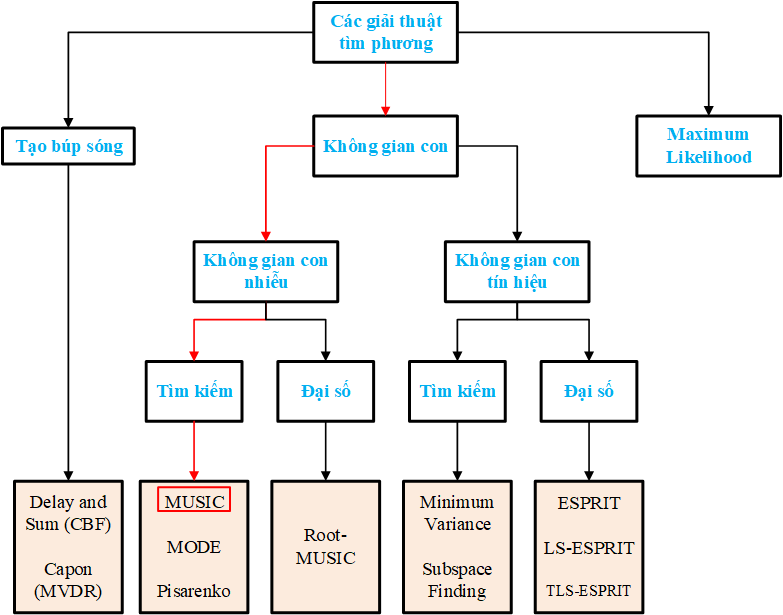
\includegraphics[width= 1\linewidth]{figures/DOA_algorithm.png}
	\caption{Các phương pháp xác định hướng sóng đến}
	\label{fig:overview}
\end{figure}

Trong hình \ref{fig:overview}, các thuật toán tìm hướng sóng đến phổ biến hiện nay được chia vào các nhóm chính, dựa trên hướng tiếp cận để giải quyết bài toán. Mục này sẽ làm nhiệm vụ giới thiệu các thuật toán tìm hướng sóng đến điển hình, mô phỏng chúng trên Matlab, qua đó đưa ra đánh giá về các ưu nhược điểm của từng thuật toán, tập trung chủ yếu vào thuật toán MUSIC sẽ sử dụng trong Chương 3.

Phương pháp thông thường để tính toán hướng sóng đến là dựa trên ý tưởng về tạo búp sóng (beamforming), không khai thác bản chất của vector tín hiệu nhận được $\mathbf{x}(k)$ hoặc mô hình thống kê tín hiệu tạp âm. Các phương pháp thông thường được trình bày dưới đây là phương pháp tạo búp sóng cổ điển (Delay and Sum) và phương pháp phương sai tối thiểu của Capon. Cùng với đó là thuật toán ML là một phương pháp tham số tìm mô hình giống nhất với tín hiệu thu được.

\subsection{Phương pháp tạo búp sóng}

\begin{figure} [!htb]
	\centering
	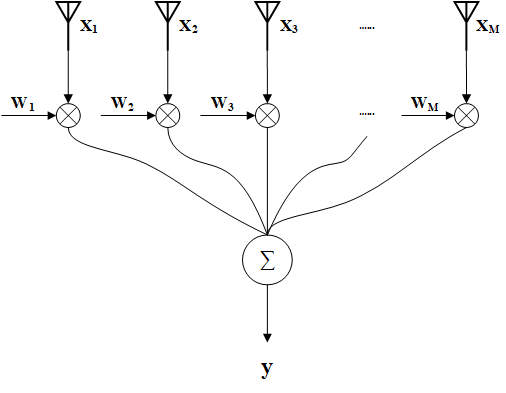
\includegraphics[width=0.7\linewidth]{figures/Beamformer.png}
	\caption{Ví dụ bộ tạo búp sóng tổng quát}
	\label{fig:beamformer}
\end{figure}

Hình \ref{fig:beamformer} biểu diễn sơ đồ bộ tạo búp sóng tổng quát băng hẹp, với tín hiệu đầu ra $\mathrm{y}(t)$ được tính bằng tổng của vector các trọng số $\mathbf{w} = [\mathrm{w}_{1}, ..., \mathrm{w}_{M}]^{T}$ nhân với các dữ liệu thu thập được từ anten.
\begin{equation}
	\mathbf{y}(t) = \mathbf{w}^{H}\mathbf{x}(t)
\end{equation}

Công suất lối ra được tính bởi:
\begin{equation}
	\mathbf{P}_{CBF}(\mathbf{w}) = E[|\mathbf{y}(t)|^{2}] = E[|\mathbf{w}^{H}\mathbf{x}(t)|^{2}] = {\mathbf{w}^{H}}E[\mathbf{x}(t)\mathbf{x}^{H}(t)]\mathbf{w} = \mathbf{w}^{H}\mathbf{R}_{\mathbf{x}}\mathbf{w}
\label{eq:Pcbf}
\end{equation}
với $\mathbf{R}_{\mathbf{x}}$ là ma trận tự tương quan lối vào. Với K mẫu $[\mathrm{y}_{1}, ..., \mathrm{y}_{K}]$, phương trình (\ref{eq:Pcbf}) trở thành:
\begin{equation}
\begin{split}
	\mathbf{P}_{CBF}(\mathbf{w}) &= \frac{1}{K}\sum_{k = 1}^{K}|\mathbf{y}(t)|^{2} = \frac{1}{K}\sum_{k = 1}^{K}\mathbf{w}^{H}\mathbf{x}(k)\mathbf{x}^{H}(k)\mathbf{w} = \mathbf{w}^{H}\tilde{\mathbf{R}}_{\mathbf{x}}\mathbf{w} \\
	\tilde{\mathbf{R}}_\mathbf{x} &= \frac{1}{K} \sum_{k = 1}^{K} \mathbf{x}(k)\mathbf{x}^{H}(k) : \text{ ước lượng của $\mathbf{R}_\mathbf{x}$}
\end{split}
\label{eq:Pcbf1}
\end{equation}

Phổ không gian của thuật toán là công suất lối ra ứng với góc quét. Các góc ứng với đỉnh trong phổ không gian chính là góc sóng đến cần ước lượng. Tới đây, việc chọn vector trọng số cho bộ tạo búp sóng được thực hiện theo nhiều phương pháp, mà dưới đây là hai phương pháp điển hình và thường xuyên được sử dụng nhất là Delay and Sum (hay bộ tạo búp sóng truyền thống) và Capon (hay bộ tạo búp sóng MVDR). 
%Chi tiết thuật toán được trình bày bên dưới:

\begin{itemize}
	\item[$\ast$] \textbf{Delay and Sum (Conventional Beamforming Method)}
\end{itemize}

Phương pháp tạo búp sóng truyền thống hay Delay-and-Sum \cite{Liberti1999} là phương pháp đơn giản nhất trong các kỹ thuật tìm hướng sóng đến bằng việc tạo búp sóng. Ý tưởng của phương pháp là quét qua các vùng góc quan tâm (thường là trong các phần rời rạc) và hướng nào tạo ra công suất đầu ra lớn nhất là được coi là hướng tín hiệu mong muốn cần ước lượng.

Xét một tín hiệu $\mathbf{x}(k)$ có hướng đến so với mảng anten thu là ${\phi}_{0}$, theo mô hình băng hẹp hình \ref{fig:beamformer} với $\mathbf{x}(t) = \sum_{k=1}^{K}\mathbf{a}_{k}(t)\mathbf{s}_{k}(t) + \mathbf{n}(t)$ (được diễn giải chi tiết ở công thức (\ref{eq:rec})), công suất đầu ra của bộ tạo búp sóng được tính bởi:
\begin{equation}
\begin{split}
	\mathbf{P}_{CBF}(\phi_{0}) &= E[|\mathbf{w}^{H}\mathbf{x}(k)|^{2}] = E[|\mathbf{w}^{H}(\mathbf{a}(\phi_{0})\mathbf{s}(k) + \mathbf{n}(k))|^{2}] \\
	&= [|\mathbf{w}^{H}\mathbf{a}(\phi_{0})|^{2}({\mathbf{\sigma}_{\mathbf{s}}}^{2} + {\mathbf{\sigma}_{\mathbf{n}}}^{2})]
\end{split}
\label{eq:barl}
\end{equation}
với $\mathbf{a}(\phi_{0})$ là vector đáp ứng mảng với sóng đến góc $\phi_{0}$, $\mathbf{n}(k)$ là vector tạp âm ở mảng đầu vào, $\sigma_{\mathbf{s}} = E[\mathbf{s}(k)^{2}]$ và $\sigma_{\mathbf{n}} = E[\mathbf{n}(k)^{2}]$ lần lượt là công suất của tín hiệu và tạp âm. Theo công thức (\ref{eq:barl}), công suất đầu ra tối đa khi $\mathbf{w} = \mathbf{a}(\phi_{0})$, hay trong tất cả các vector trọng số có thể, anten thu có mức tăng cao nhất theo hướng $\phi_{0}$ khi $\mathbf{w} = \mathbf{a}(\phi_{0})$. Điều này có được do $\mathbf{w} = \mathbf{a}(\phi_{0})$ căn chỉnh góc của các thành phần tín hiệu đến từ góc $\phi_{0}$ tại mảng anten thu, vậy nên chúng đẩy giá trị công suất lên.

Thay $\mathbf{w} = \mathbf{a}(\phi_{0})$ vào công thức của công suất lối ra ứng với góc quét (\ref{eq:Pcbf1}), phổ không gian vẽ bởi công suất lối ra từ bộ tạo búp sóng truyền thống tương ứng:
\begin{equation}
	\mathbf{P}_{CBF}(\phi) =\mathbf{w}^{H}\tilde{\mathbf{R}}_{\mathbf{x}}\mathbf{w} = \mathbf{a}^{H}(\phi)\tilde{\mathbf{R}}_{\mathbf{x}}\mathbf{a}(\phi)
\end{equation}

Vì là phương pháp đơn giản nhất nên phương pháp tạo búp sóng truyền thống có nhiều nhược điểm: độ rộng của búp sóng lớn dẫn đến khi có nhiều nguồn đến với góc gần nhau, công suất của chúng sẽ bị cộng lại thành một búp sóng duy nhất. Mặc dù có thể tăng độ phân giải bằng cách tăng số lượng máy thu nhưng cách tốt hơn là sử dụng một thuật toán tạo búp sóng khác, đó là Capon được trình bày dưới đây.

\begin{itemize}
	\item[$\ast$] \textbf{Thuật toán tạo búp sóng của Capon}
\end{itemize}

Bộ tạo búp sóng Capon \cite{Capon2009} hay Minimum Variance Distortionless Response cũng là một phương pháp phổ biến để khắc phục hạn chế về độ phân giải của phương pháp CBF. Phương pháp này thực hiện tối thiểu hóa công suất tạp âm và công suất theo các hướng khác, ngoại trừ hướng của tín hiệu đến $\phi_{0}$ vì vậy vector trọng số $\mathbf{w}$ trong phương trình (\ref{eq:capon}) còn được gọi là vector trọng số của búp sóng đáp ứng không méo phương sai tối thiểu (MVDR). Phương pháp này có phương trình tối ưu:
\begin{equation}
	\underset{\mathbf{w}}{\mathbf{min}}\; E[|\mathbf{y}(k)|^{2}] = \underset{\mathbf{w}}{\mathbf{min}}\; \mathbf{w}^{H}\mathbf{R}_{\mathbf{x}}\mathbf{w} \;\;\textrm{với}\;\; \mathbf{w}^{H}\mathbf{a}(\phi_{0}) = 1
\label{eq:capon} 
\end{equation}

Sử dụng phương pháp nhân tử Lagrange,  giải được nghiệm của phương trình (\ref{eq:capon}) là vector trọng số:
\begin{equation}
	\mathbf{w} = \frac{{\mathbf{R}_{\mathbf{x}}}^{-1}\mathbf{a}(\phi)}{\mathbf{a}^{H}(\phi){\mathbf{R}_{\mathbf{x}}}^{-1}\mathbf{a}(\phi)}
\end{equation}

Với nghiệm trên, thay vào (\ref{eq:Pcbf1}), phổ không gian vẽ bởi công suất lối ra từ bộ tạo búp sóng Capon, với các đỉnh của phổ không gian chính là ước lượng hướng sóng đến của tín hiệu tương ứng:
\begin{equation}
	\mathbf{P}_{Capon}(\phi) = \frac{1}{\mathbf{a}^{H}(\phi)\mathbf{R}_{\mathbf{x}}\mathbf{a}(\phi)}
\end{equation}

Hình \ref{fig:CBFvsCapon} là kết quả mô phỏng 2 thuật toán tìm hướng sóng đến CBF và Capon trên Matlab với 2 nguồn phát ở góc 80$^{\circ}$ và 85$^{\circ}$, mảng anten thu gồm 4 phần tử anten đặt thẳng cách đều nhau  $0,5\lambda = 0,5 \times 0,325 (m)$. Có thể thấy phương pháp CBF chỉ nhận diện được một búp sóng ở khoảng góc từ 60$^{\circ}$ đến 100$^{\circ}$ còn Capon đã khắc phục được độ phân giải kém này khi xác định được 2 đỉnh ở 80$^{\circ}$ và 85$^{\circ}$. Tuy nhiên, dễ nhận thấy khi góc đến thu hẹp hơn nữa chỉ 1$^{\circ}$ hay 2$^{\circ}$ thì phương pháp Capon cũng khó có thể phân biệt được. Hơn nữa, phương pháp Capon cần có điều kiện là không có các tín hiệu khác tương quan với tín hiệu cần xác định hướng sóng đến và trong thuật toán có phương trình yêu cầu nghịch đảo ma trận, nếu tăng số phần tử thu lớn có thể dẫn đến tốn kém bộ nhớ.
\begin{figure} [!htb]
	\centering
	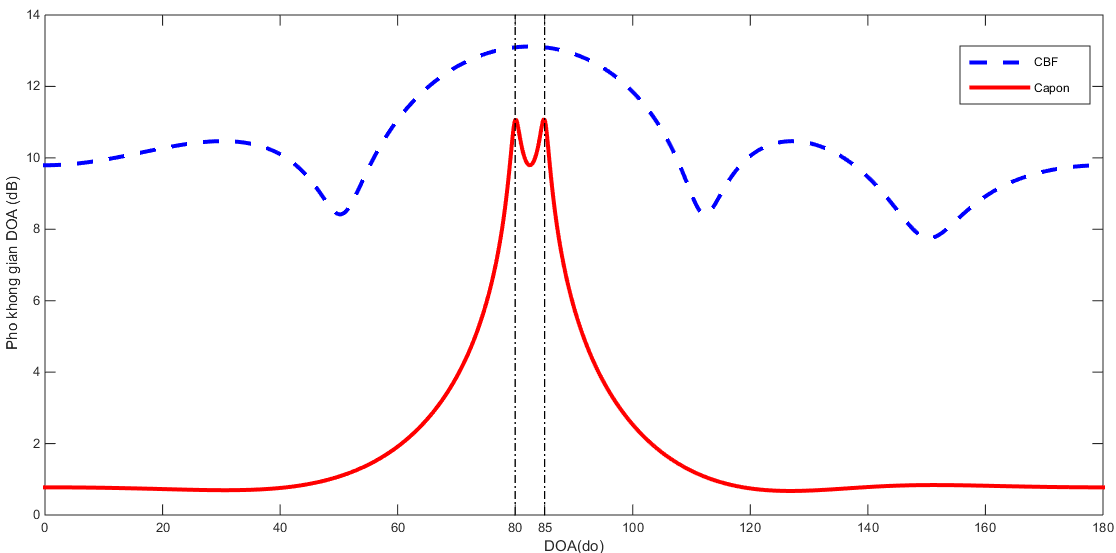
\includegraphics[width=1\linewidth]{figures/CBFvsCapon.png}
	\caption{Mô phỏng thuật toán Delay and Sum và Capon}
	\label{fig:CBFvsCapon}
\end{figure}

\subsection{Thuật toán Maximum Likelihood}

Maximum Likelihood (ML) là một trong những thuật toán đầu tiên được phát triển để tính toán DOA. Tuy không phổ biến bằng thuật toán MUSIC trình bày trong mục 1.3 bên dưới, tuy nhiên do sử dụng phương pháp tham số nên tránh được các vấn đề nhiễu đa đường, tín hiệu tương quan cao, số lượng mẫu nhỏ của các phương pháp dùng phổ \cite{Ziskind1988}.

Với nguyên tắc cơ bản là tìm mô hình dữ liệu giống nhất với dữ liệu được thu thập tại mảng anten thu. Vẫn tiếp tục sử dụng mô hình tín hiệu nguồn như phương trình (\ref{eq:rec}), hàm mật độ xác suất chung của K mẫu thu thập $\mathbf{x}(1), ..., \mathbf{x}(K)$  là:
\begin{equation}
	\mathit{f}(\mathbf{x}) = \prod_{k=1}^{K}\frac{1}{\pi\mathbf{det}[\sigma^2\mathbf{I}]} \cdot  \mathrm{exp}(-\frac{1}{\sigma^2}|\mathbf{x}(k) - A(\Phi)\mathbf{s}(k)|^2)
\end{equation}
với $\mathbf{det}$ là định thức của ma trận. Tiếp theo, loại bỏ các thành phần không phụ thuộc vào $\Phi$, ta có hàm  log likelihood:
\begin{equation}
	L(\Phi) = -Mp\log\sigma^2 - \frac{1}{\sigma^2}\sum_{k=1}^{K}|\mathbf{x}(k) - A(\Phi)\mathbf{s}(k)^2|
\end{equation}

Phương pháp ML thực hiện tìm giá trị cực đại của hàm log likelihood khi thay đổi các giá trị $\Phi$ và $\mathbf{s}$, bỏ qua các giá trị không thay đổi, ta thu được:
\begin{equation}
	\underset{\Phi, \mathbf{s}}{\max} \left[-Mp\log(\frac{1}{Mp}\sum_{k=1}^{K}|\mathbf{x}(k) - A(\Phi)\mathbf{s}(k)|^2)\right]
\label{eq:ML}
\end{equation}

Do $\mathbf{log}$ là một hàm đơn điệu nên tìm cực đại của phương trình (\ref{eq:ML}) tương đương với:
\begin{equation}
	\underset{\Phi, \mathbf{s}}{\min} \left[\sum_{k=1}^{K}|\mathbf{x}(k) - A(\Phi)\mathbf{s}(k)|^2\right]
\label{eq:ML1}
\end{equation}

Các bước tiếp thuộc vấn đề tối ưu hóa phi tuyến tính nhiều chiều và phức tạp, cụ thể được trình bày ở \cite{Ziskind1988}.

\section{Hệ thống xác định hướng sóng đến với thuật toán MUSIC}

Phương pháp phương sai tối thiểu của Capon thường chính xác và được sử dụng rộng rãi, tuy nhiên phương pháp này có một số hạn chế cơ bản trong độ phân giải. Còn phương pháp tham số: ML lại có độ phức tạp cao khi thực hiện tìm kiếm D-D (D chiều). Schmidt đã đưa ra một giải pháp hoàn chỉnh dựa trên thống kê bậc hai cho vấn đề ước lượng DOA, có khả năng áp dụng cho mọi loại tín hiệu với cấu trúc anten tùy ý. Kỹ thuật được đề xuất bởi Schmidt vào năm 1979 với tên gọi: thuật toán phân loại đa tín hiệu (MUSIC) \cite{Schmidt2009a}. Sơ đồ khối của hệ tìm hướng sóng đến sử dụng thuật toán MUSIC được đưa ra trên hình \ref{fig:musicstruct}.

\begin{figure} [!h]
	\centering
	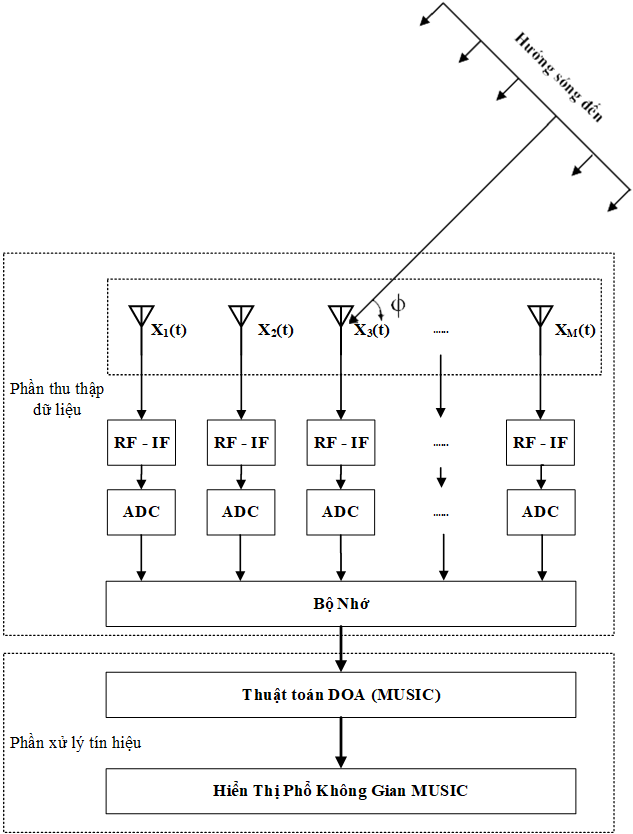
\includegraphics[width=0.75\linewidth]{figures/MuSIC_Structor.png}
	\caption{Sơ đồ khối hệ tìm hướng sóng đến sử dụng thuật toán MUSIC}
	\label{fig:musicstruct}
\end{figure}

Xét D nguồn tín hiệu đến với các hướng không biết trước $\phi_{1}$, ..., $\phi_{D}$ đến mảng anten thu gồm M (điều kiện M > D) phần tử vô hướng được đặt tùy ý trong mặt phẳng ở các tọa độ ($\bar{\mathrm{x}}_1$, $\bar{\mathrm{y}}_1$), ..., ($\bar{\mathrm{x}}_M$, $\bar{\mathrm{y}}_M$).

Vector tín hiệu bên thu nhận được $\mathbf{x}(t) \in \mathbb{C}^{M}$  tại thời điểm \textit{t} được biểu diễn bởi công thức (\ref{eq:rec}), với $\Phi$ = $[\phi_{1}, ..., \phi_{D}]^{T}$ tương ứng với hướng của các nguồn tín hiệu đến mảng anten thu, $\mathbf{A}(\Phi) = [\mathbf{a}(\phi_{1}), ..., \mathbf{a}(\phi_{D})] \in \mathbb{C}^{M  \times D}$ là mà trận chứa các vector đáp ứng mảng $\mathbf{a}(\phi) \in \mathbb{C}^{M}$; $\mathbf{s}(t) \in \mathbb{C}^{D}$ là vector nguồn tín hiệu và $\mathbf{n}(t) \in \mathbb{C}^{M}$ tương ứng là vector tạp âm:
\begin{equation}
\begin{matrix}
\begin{bmatrix}
\mathrm{x}_{1}(t) \\
... \\
\mathrm{x}_{M}(t)
\end{bmatrix}
=
\begin{bmatrix}
 &  & \\ 
\mathbf{a}(\phi_{1}) &...  &\mathbf{a}(\phi_{D})\\ 
 &  & 
\end{bmatrix}
\begin{bmatrix}
\mathrm{s}_{1}(t)\\ 
...\\ 
\mathrm{s}_{D}(t)
\end{bmatrix}
+
\begin{bmatrix}
\mathrm{n}_{1}(t)\\ 
...\\ 
\mathrm{n}_{M}(t)
\end{bmatrix}\\  
\\ \textrm{hay được viết dưới dạng ma trận}\\ \\
\mathbf{x}(t) = \mathbf{A}(\Phi)\mathbf{s}(t) + \mathbf{n}(t)\\ 
\end{matrix}
\label{eq:rec}
\end{equation}

Trong đó, vector đáp ứng mảng được biểu diễn chi tiết như công thức (\ref{eq:resp}) với $\lambda$ là bước sóng của tín hiệu:
\begin{equation}
\mathbf{a}(\phi) = 
\begin{bmatrix}
e^{-j\frac{2\pi}{\lambda}(\bar{\mathrm{x}}_{1}\cos\phi \,+\, \bar{\mathrm{y}}_{1}\sin\phi)}\\ 
...\\ 
e^{-j\frac{2\pi}{\lambda}(\bar{\mathrm{x}}_{M}\cos\phi \,+\, \bar{\mathrm{y}}_{M}\sin\phi)}
\end{bmatrix}
\label{eq:resp}
\end{equation}

Các vector đáp ứng mảng này là các giá trị cần được giả thiết là biết trước tùy theo cấu hình anten, được lưu trữ làm các giá trị chuẩn hóa cần thiết cho mọi bước tính toán; vector tín hiệu và tạp âm (nhiễu trắng) có trung bình bằng 0; vector tạp âm trắng hóa không gian (tạp âm đến mỗi phần tử anten đều có phương sai giống nhau là ${\sigma_{\mathrm{n}}}^{2}$ không tương quan với nhau) và độc lập thống kê với các tín hiệu nguồn.

Ma trận hiệp phương sai trong không gian được biểu diễn bởi công thức (\ref{eq:Ruu}), với $\mathcal{E}$ là ký hiệu của kỳ vọng thống kê, $\mathcal{E}\{\mathbf{s}(t)\mathbf{s}^{H}(t)\} = \mathbf{R}_{\textbf{s}}$, $\mathcal{E}\{\mathbf{n}(t)\mathbf{n}^{H}(t)\} = \mathbf{{{\sigma}_{\mathrm{n}}}^{2}I_{\mathbf{n}}}$ lần lượt là ma trận tương quan của tín hiệu nguồn và của tạp âm, $\mathbf{{I_{n}}} \in \mathbb{C}^{M \times M}$ là ma trận đơn vị. 
\begin{equation}
\begin{split}
	\mathbf{C}_{\mathbf{x}} = \mathbf{R}_{\mathbf{x}} &= 	\mathcal{E}\{\mathbf{x}(t)\mathbf{x}^{H}(t)\}	\\
	&= \mathbf{A}\mathcal{E}\{\mathbf{s}(t)\mathbf{s}^{H}(t)\}\mathbf{A}^{H} + \mathcal{E}\{\mathbf{n}(t)\mathbf{n}^{H}(t)\}	\\
	&= \mathbf{A}\mathbf{R}_{\mathbf{s}}\mathbf{A}^{H} + {\sigma_{\mathbf{n}}}^{2}\mathbf{I}_{\mathbf{n}}
\end{split}
\label{eq:Ruu}
\end{equation}

Tiếp tục khai triển ma trận $\mathbf{R}_{\mathbf{x}}$ thành các giá trị riêng và các vector riêng tương ứng là $\lambda_{m}$ và $\mathbf{e}_{m} (m =1, ..., M)$.
\begin{equation}
\begin{split}
	\mathbf{R}_{\mathbf{x}} &= \sum_{m = 1}^{M} \lambda_{m}\mathbf{e}_{m}{\mathbf{e}_{m}}^{H} = \mathbf{E}\Lambda\mathbf{E}^{H} = \mathbf{E}_{\mathbf{s}}\Lambda_{\mathbf{s}}{\mathbf{E}_{\mathbf{s}}}^{H} + \mathbf{E}_{\mathbf{n}}\Lambda_{\mathbf{n}}{\mathbf{E}_{\mathbf{n}}}^{H} \\
	  &=\mathbf{E}_{\mathbf{s}}\Lambda_{\mathbf{s}}{\mathbf{E}_{\mathbf{s}}}^{H} +  {\mathbf{\sigma}_{\mathbf{n}}}^{2}\mathbf{E}_{\mathbf{n}}{\mathbf{E}_{\mathbf{n}}}^{H} = \mathbf{E}_{\mathbf{s}}\tilde{\Lambda}_{\mathbf{s}}{\mathbf{E}_{\mathbf{s}}}^{H} + {\mathbf{\sigma}_{\mathbf{n}}}^{2}\mathbf{I}_{\mathbf{n}}
\end{split}
\end{equation}
{\renewcommand\labelitemi{}
\begin{itemize}
  \item với $\mathbf{E} = [\mathbf{e}_{1}, ..., \mathbf{e}_{M}]$
  \item \hspace{0.7cm}$\mathbf{E}_{\mathbf{s}} = [\mathbf{e}_{1}, ..., \mathbf{e}_{D}]$
  \item \hspace{0.7cm}$\mathbf{E}_{\mathbf{n}} = [\mathbf{e}_{D+1}, ..., \mathbf{e}_{M}]$ 
  \item \hspace{0.7cm}$\Lambda = diag\{\lambda_{1}, ..., \lambda_{M}\}$
  \item \hspace{0.7cm}$\Lambda_{\mathbf{s}} = diag\{\lambda_{1}, ..., \lambda_{D}\}$
  \item \hspace{0.7cm}$\Lambda_{\mathbf{n}} = diag\{\lambda_{D}, ..., \lambda_{M}\}$
  \item \hspace{0.7cm}$\tilde{\Lambda}_{\mathbf{s}} = \Lambda_{\mathbf{s}} - {\mathbf{\sigma}_{\mathbf{n}}}^{2}\mathbf{I}_{\mathrm{n}}$
\end{itemize}
}
 
Vector riêng $\mathbf{E} = [\mathbf{E}_{\mathbf{s}}, \mathbf{E}_{\mathbf{n}}]$ có thể giả sử để tạo thành một cơ sở trực giao ($\mathbf{E}\mathbf{E}^{H} = \mathbf{E}^{H}\mathbf{E} = \mathbf{I})$. Từ $\mathbf{E}$ có thể tách được ra hai ma trận: ma trận chứa D vector riêng tương ứng với không gian con tín hiệu là $\mathbf{E}_{\mathbf{s}} \triangleq [\mathbf{e}_{1}, ..., \mathbf{e}_{D}]$; ma trận chứa M - D vector riêng tương ứng với không gian con của tạp âm là $\mathbf{E}_{\mathbf{n}} \triangleq [\mathbf{e}_{D+1}, ..., \mathbf{e}_{M}]$. Để phân tích chi tiết các thuộc tính cấu trúc riêng của ma trận hiệp phương sai $\mathbf{R}_{\mathbf{x}}$ tham khảo tại \cite{Schmidt2009a}.


Khi các không gian con đã được xác định, có thể ước tính hướng đến của các tín hiệu mong muốn bằng cách tính phổ không gian MUSIC trên vùng quan tâm:
\begin{equation}
	\mathbf{P}_{MUSIC}(\phi) = \frac{\mathbf{a}^{H}(\phi)\mathbf{a}(\phi)}{\mathbf{a}^{H}(\phi)\mathbf{E}_{\mathbf{n}}{\mathbf{E}_{\mathbf{n}}}^{H}\mathbf{a}({\phi})}
\end{equation}

Thực hiện mô phỏng với thông số mảng thu tương tự như thuật toán Capon trên Matlab, tuy nhiên thay đổi góc của 2 nguồn tín hiệu phát là 80$^{\circ}$ và 82$^{\circ}$, hình \ref{fig:MUSICvsCapon} dưới đây biểu diễn kết quả thu được. Có thể thấy rõ sự vượt trội của thuật toán MUSIC trong việc ước tính DOA.
\begin{figure} [!htb]
	\centering
	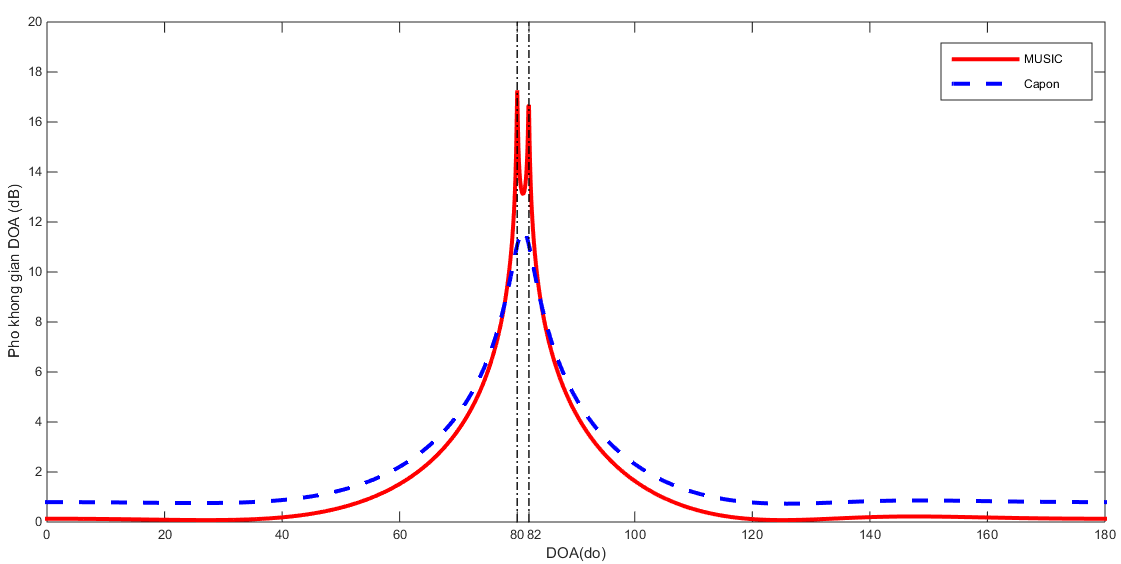
\includegraphics[width=1\linewidth]{figures/MUSICvsCapon.png}
	\caption{Mô phỏng thuật toán MUSIC và Capon}
	\label{fig:MUSICvsCapon}
\end{figure}
